\section{The Simpsons} \label{P2}
\subsubsection*{The TV Show}
\begin{figure}[!htb]
    \centering
    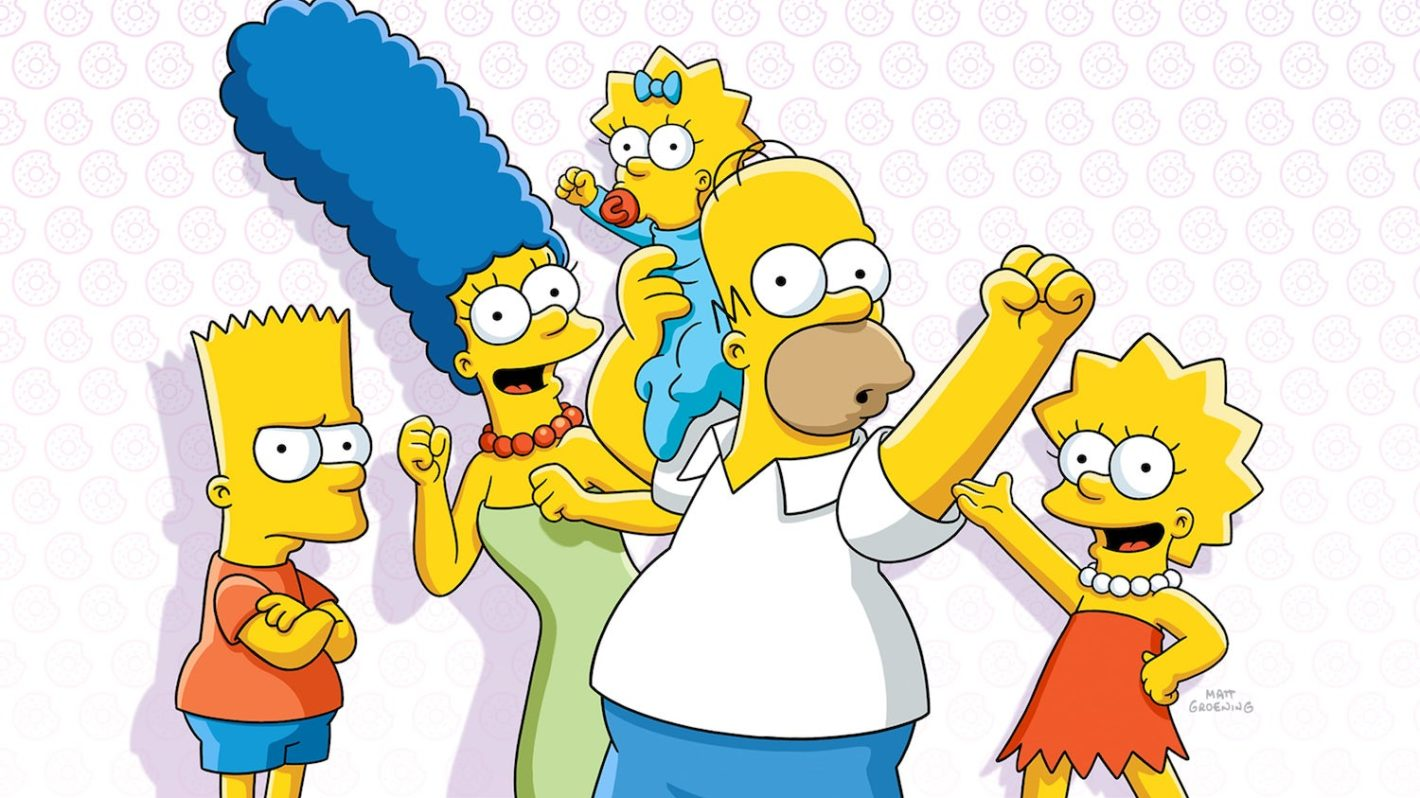
\includegraphics[width=0.95\linewidth]{Resources/simpson.jpg}
    \caption{Simpsons}
    \label{fig:P1Q3b}
\end{figure}

The Simpsons is an American animated sitcom created by Matt Groening for the Fox Broadcasting Company The series is a satirical depiction of American life, epitomized by the Simpson family, which consists of Homer, Marge, Bart, Lisa, and Maggie. The show is set in the fictional town of Springfield and parodies American culture and society, television, and the human condition.

The family was conceived by Groening shortly before a solicitation for a series of animated shorts with producer James L. Brooks. He created a dysfunctional family and named the characters after his own family members, substituting Bart for his own name; he thought Simpson was a funny name in that it sounded similar to "simpleton". The shorts became a part of The Tracey Ullman Show on April 19, 1987. After three seasons, the sketch was developed into a half-hour prime time show and became Fox's first series to land in the Top 30 ratings in a season (1989–1990).

Since its debut on December 17, 1989, 728 episodes of the show have been broadcast. It is the longest-running American animated series, longest-running American sitcom, and the longest running American scripted prime time television series, both in terms of seasons and number of episodes. A feature-length film, The Simpsons Movie, was released in theaters worldwide on July 27, 2007, and grossed over \$527 million, with a sequel in development as of 2018. The series has also spawned numerous comic book series, video games, books, and other related media, as well as a billion-dollar merchandising industry. The Simpsons is a joint production by Gracie Films and $20^{th}$ Television. On March 3, 2021, the series was announced to have been renewed for seasons 33 and 34, which were later confirmed to have 22 episodes each, increasing the episode count from 706 to 750. Its thirty-third season premiered on September 26, 2021.

The Simpsons received acclaim throughout its early seasons in the 1990s, which are generally considered its "golden age". Since then, it has been criticized for a perceived decline in quality. Time named it the $20^{th}$ century's best television series, and Erik Adams of The A.V. Club named it "television's crowning achievement regardless of format". On January 14, 2000, the Simpson family was awarded a star on the Hollywood Walk of Fame. It has won dozens of awards since it debuted as a series, including 34 Primetime Emmy Awards, 34 Annie Awards, and 2 Peabody Awards. Homer's exclamatory catchphrase of "D'oh!" has been adopted into the English language, while The Simpsons has influenced many other later adult-oriented animated sitcom television series.
\parencite{simpsons}